%!TEX root = ../main.tex

\graphicspath{{./figures/chapter2/}}


\chapter{Single RNA Detection} \label{ch:chapter2}
\minitoc
\newpage

In this chapter we review different techniques for spot detection.
Even though the problem is not new, and has been largely addressed by different scientific communities, none of the suggested methods really meet the requirements of a high content screening analysis with \ac{FISH} experiments.

The second part of this chapter therefore describe our own implementation in \mbox{\emph{bigfish.detection}}.
We try to answer specific limitations of existing solutions, especially the possibility to scale the detection.
As an example, we also add a code snippet at the end of each step.

Finally we evaluate the robustness and the accuracy of our implementation by simulating spots under different noise conditions.

\section{Spot detection as a signal processing problem} \label{sec:detection_introduction}

We first describe inputs and outputs we can expect when we perform spot detection.
Then we review some solutions proposed in the literature, in bio-informatics, but more generally in computer vision.
Lastly, we briefly discuss two recent methods based on a deep-learning framework.

\begin{figure}[h]
    \centering
    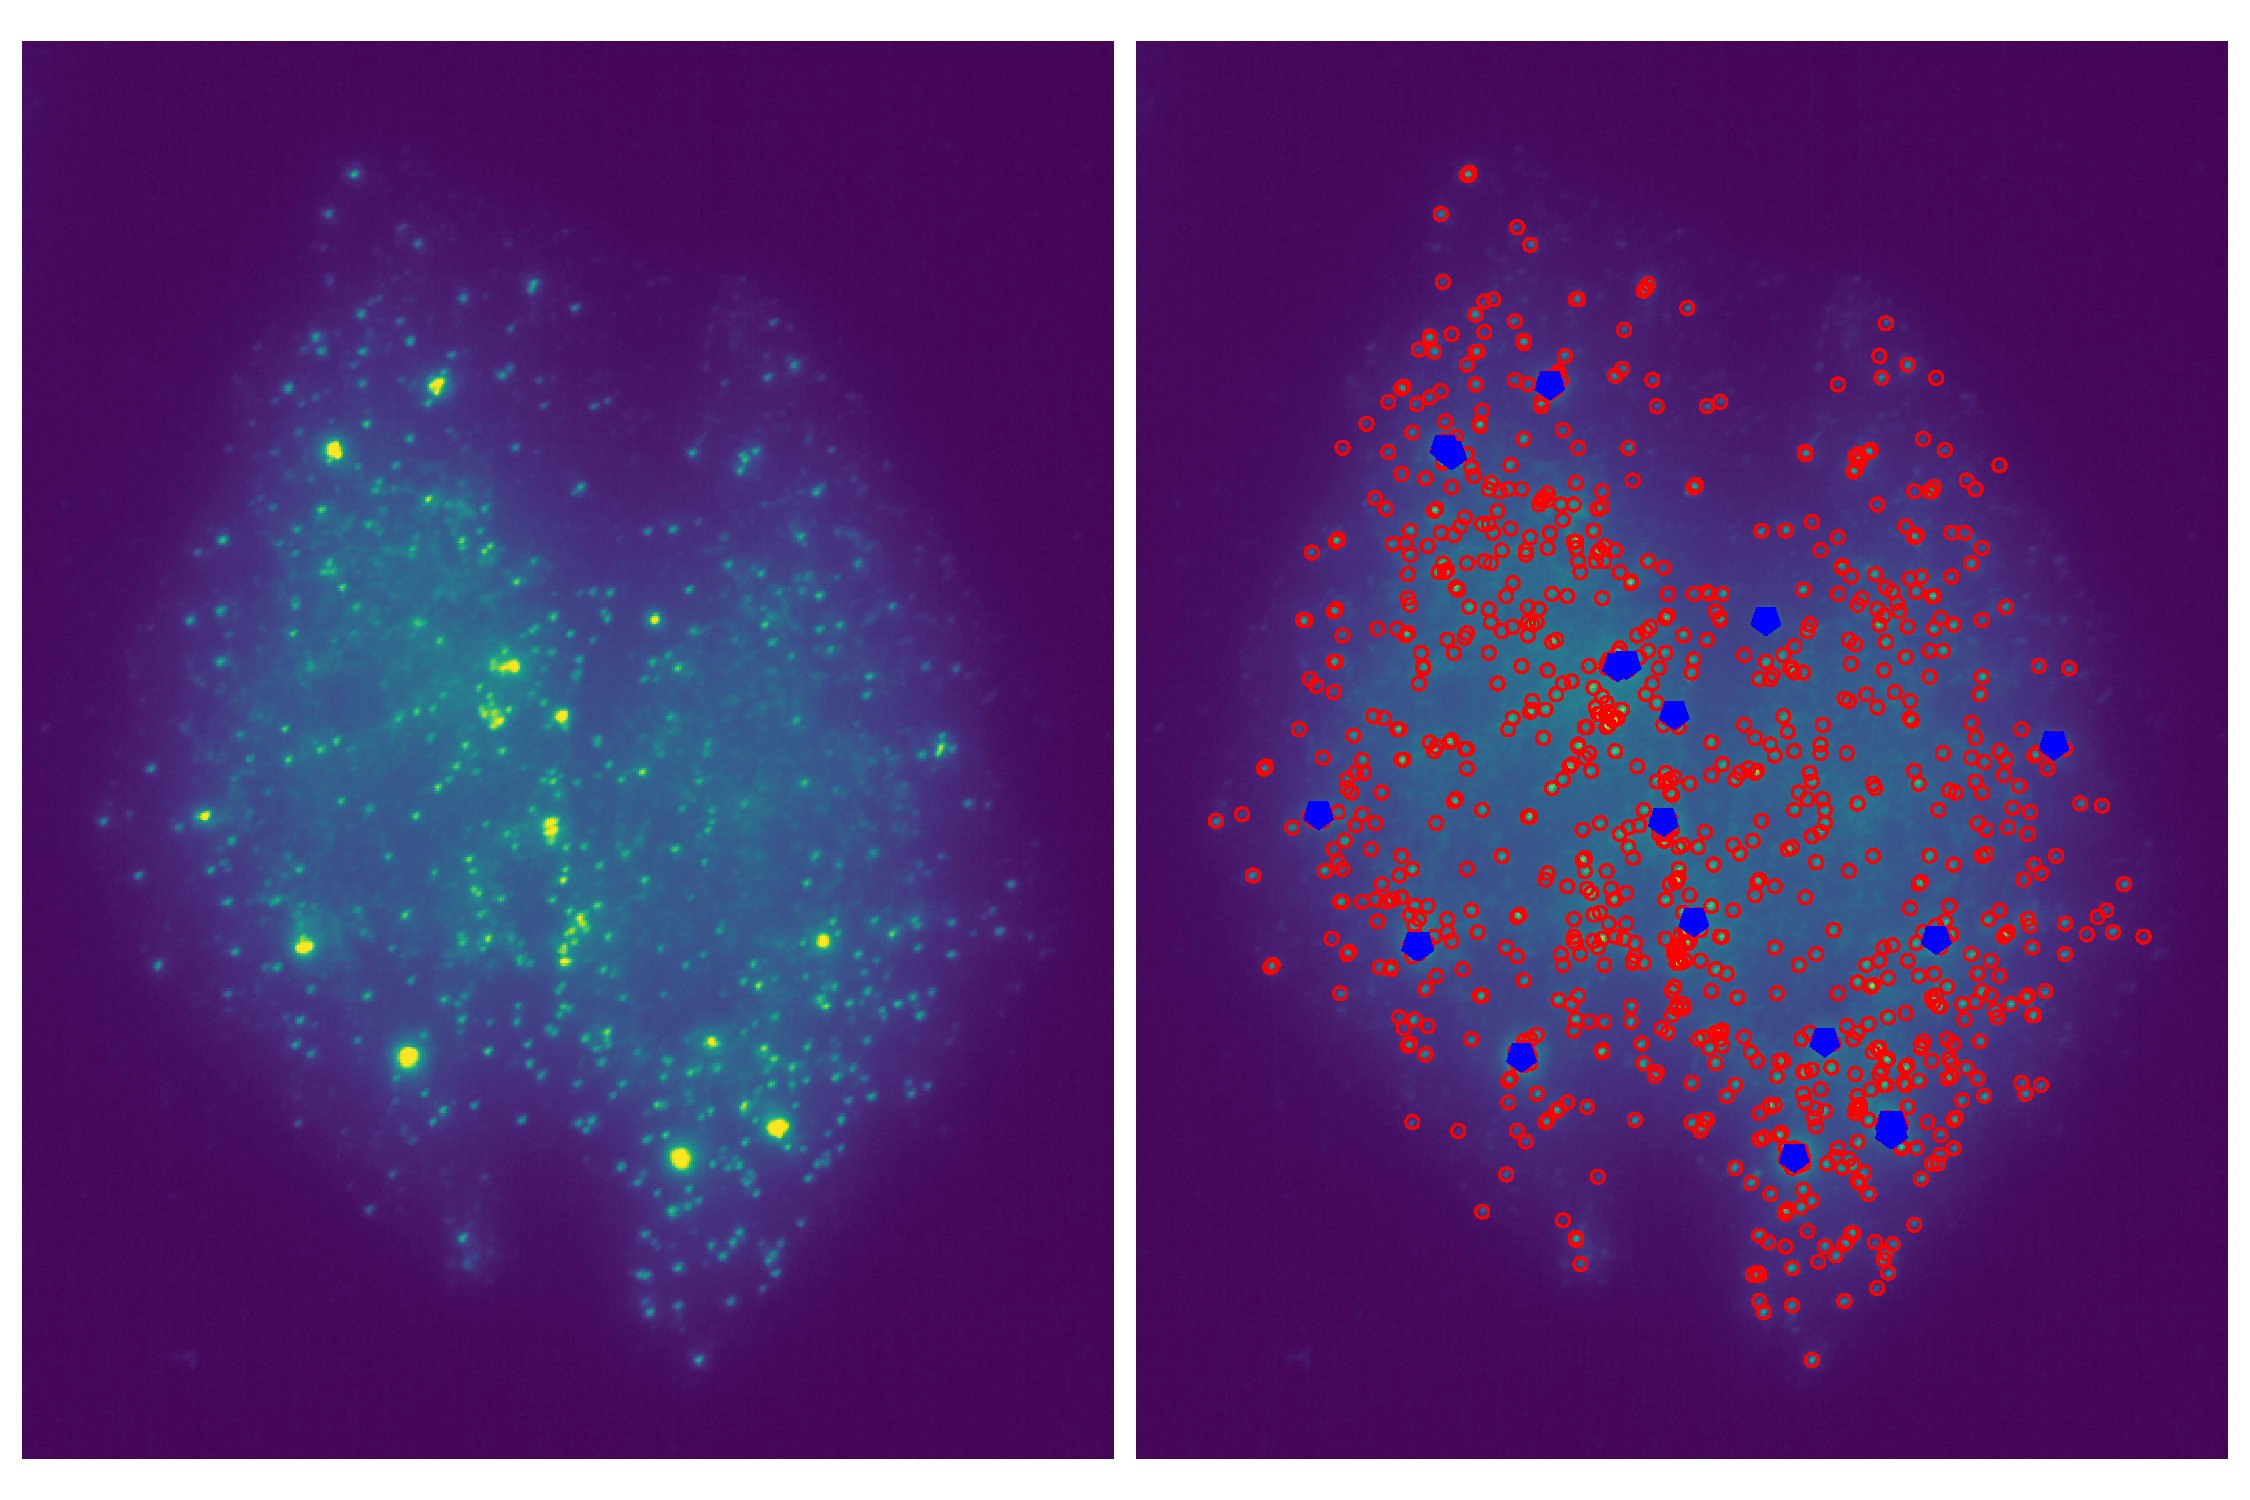
\includegraphics[width=1\textwidth]{figures/chapter2/cluster_detection_results}
    \caption{Spot (red) and cluster (blue) detection with \emph{bigfish.detection}}
    \label{fig:detection_results}
\end{figure}

\subsection{Extract spot coordinates from an image} \label{subsec:detection}

Aim of spot detection is to extract a array of spatial coordinates from an image with identifiable point sources.
This task is performed in two or three dimensions, depending of the input image.

Detecting an object as small as a \ac{RNA} molecule implies some constraints.
The optical system does not capture the original light signal emitted by the fluorescence probes, but its convolution with a \ac{PSF}.
However, for the rest of the chapter, we simply assume the resulting spot signal can be approximate by a gaussian signal.
Such simplification is reasonable for a detection with a pixel accuracy, with our noise level.
In addition, as we can observe in figure~\ref{fig:detection_results}, a \ac{smFISH} image often present a background fluorescence that doesn't identify with a \ac{RNA}.
The noise can be highly heterogeneous and vary between images and even cells.\\

\noindent
We can observe two types of noise:
\begin{itemize}
	\item At the \ac{FoV} level, the noise from the optical setup itself and the experimental conditions.
	\item At the cellular level, the difference in the autofluorescence of the observed samples.
\end{itemize}

In the context of a high content screening study, numerous images are acquired, with various biological samples or conditions.
This leads to potentially heterogeneous pixel intensity and spot distribution across different images.
Spot detection can be really challenging.
It thus requires a robust approach to tackle this problem and extract accurate coordinates.

\subsection{Related work} \label{subsec:detection_related_work}

%The second step, fluorescence spot detection, has been addressed by a number
%of approaches in the lit- erature, and more recently solutions specifically
%adapted to smFISH have been proposed. RS-FISH allows robust and accurate detection
%of fluorescent spots in 2D and 3D through radial symmetry but requires parameter
%tuning before being scaled to a large set of images (Bahry et al. 2021). DeepLink
%is a parameter-free deep-learning-based method, but is currently only available
%for 2D data and might require retraining (Eichenberger et al. 2021). Lastly,
%assigning spot counts to segmentation results and the subsequent analysis of
%RNA levels and/or RNA locali- zation requires custom-written code (Stoeger et al. 2015; Samacoits et al. 2018).

% general review
% reference blob detection (scikit-image)
% reference Astropy
% reference RS-FISH

\subsection{Learning to spot} \label{subsec:detection_dl}

% reference DeepSpot
% reference DeepBlink

\section{Scaling \ac{mRNA} detection} \label{sec:method}

We now describe at depth the algorithms currently implemented in \emph{bigfish.detection}.

\subsection{Spot detection} \label{subsec:spot_detection}

The method we use is directly adapted from the original version of FISH-quant\cite{mueller_fish-quant_2013} and the blob detection algorithms\cite{walt_scikit-image_2014}.
Detection is performed in 2D or 3D. Image is filtered in order to increase its \ac{SNR}, then each spot is defined as a local maximum above a specific threshold.

\paragraph{Filtering}

We apply a \ac{LoG} filter (one Gaussian filter followed by a Laplacian one).
It's a two-step algorithm that enhances the spot signals.
The first Gaussian filter smooths the image and removed the high frequency noise.
The second Laplacian filter approximates the second derivative of the image.
We apply this operator at a single scale because we assume an unique size for the spots.
By default, the size of the Gaussian kernel is set to match the expected size of the spot.
The latter is assumed to be known for a given experiment and should not prevent the user to scale the detection.
If we consider a 2D image $f(x,y)$, the \ac{LoG} filter consists in computing the second derivative of the smoothed image $L(x, y, \sigma^2)$:

\begin{equation}
	\nabla^{2}L(x, y, \sigma^2) = \frac{\partial^{2}L(x, y, \sigma^2)}{\partial x^2} + \frac{\partial^{2}L(x, y, \sigma^2)}{\partial y^2}
\end{equation}

\noindent
with $L(x, y, \sigma^2)$ the convolve image:

\begin{equation}
	L(x, y, \sigma^2) = g(x, y, \sigma^2) * f(x, y)
\end{equation}

\noindent
and $g(x, y, \sigma^2)$ the Gaussian kernel with a scale $\sigma^2$:

\begin{equation}
	g(x, y, \sigma^2) = \frac{1}{2\pi \sigma^2} e^{-{\frac{x^{2} + y^{2}}{2\sigma^2}}}
\end{equation}

An alternative filter is the \ac{DoG} filter.
We estimate the background of the image with a large Gaussian kernel, then we subtract it from the original image or one smoothed with a narrower Gaussian kernel.
It is a fast approximation of the \ac{LoG} filter.
As illustrated in figure~\ref{fig:filters_detection}, both methods aim to remove the background signal and increase the \ac{SNR} of the spots.

% reference LoG and DoG

\begin{figure}[h]
    \centering
    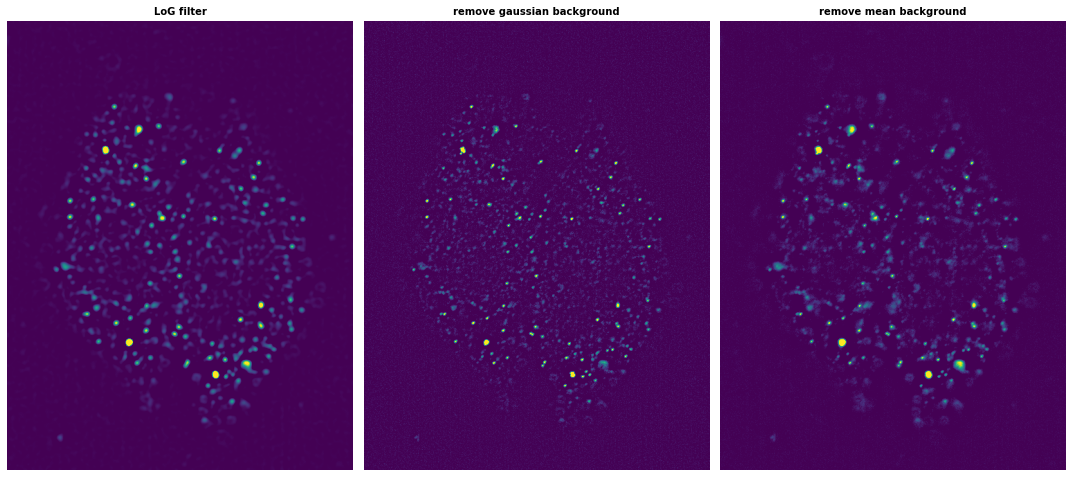
\includegraphics[width=1\textwidth]{figures/chapter2/filter_background}
    \caption{\ac{LoG} filter (left) and \ac{DoG} filter (right)}
    \label{fig:filters_detection}
\end{figure}

\paragraph{Peak detection}

A Local Maximum detection algorithm follows the filtering.
We apply a maximum filter on the \ac{LoG}-filtered image and compare the result to the original one.
A pixel with the same value in the original and filtered images is defined as a local maximum.
If, by chance, a spot has several identical pixels at its peak, we only keep one to define the spot coordinate.

% reference local maximum algorithm

\paragraph{Thresholding}

% partially copy paste from paper supplementary (Imbert et al, 2022)
At this stage, actual spots and noisy fluorescent blobs (autofluorescence, of-site binding of oligos, etc.) are both detected.
From all previously detected local peaks, we only keep those above a specific threshold.
A first limitation of spot detection algorithm appears with the choice of this threshold.
If it is manually set, it might be difficult to scale the method to a large experiment as the fluorescence can be quite heterogeneous between images.
Thus, we use a heuristic technique to set a threshold per image in a automated way.

\begin{wrapfigure}{L}{0.35\textwidth}
  \begin{center}
    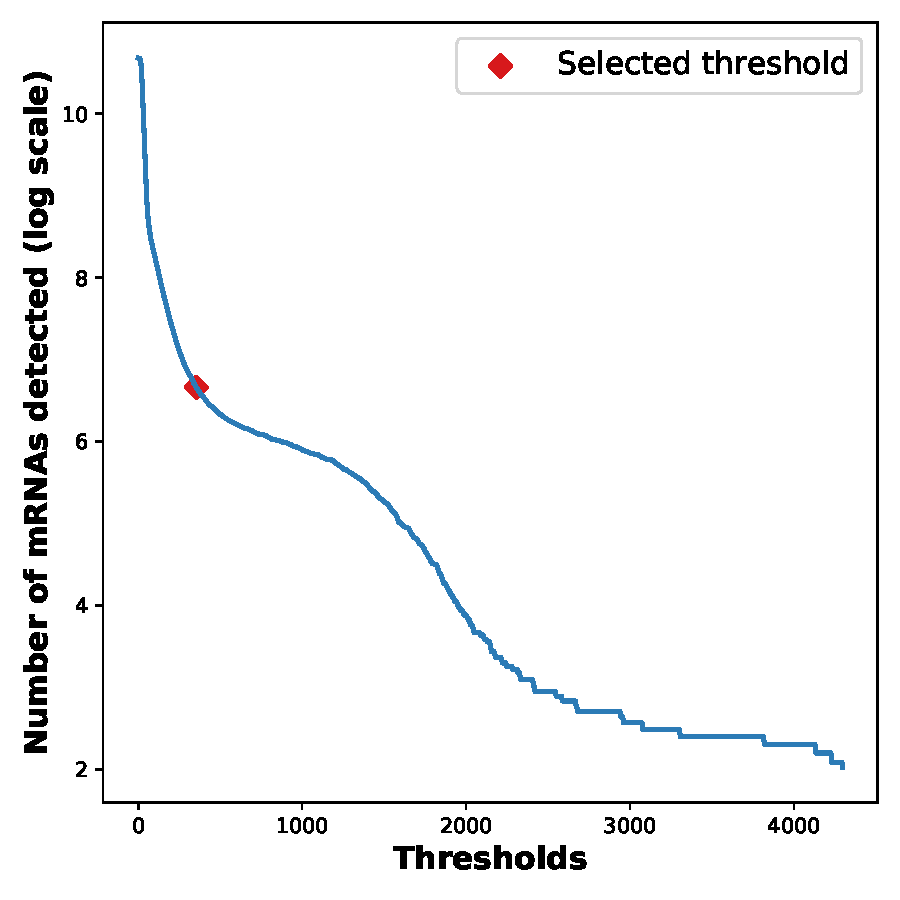
\includegraphics[width=0.33\textwidth]{figures/chapter2/elbow_curve_real}
  \end{center}
  \caption{Elbow curve}
  \label{fig:elbow_detection}
\end{wrapfigure}

We assume that a \ac{mRNA} spot and a background fluorescent noise have different intensity distribution.
The former have significantly higher intensity values since a \ac{mRNA} molecule is targeted by multiple oligos.
In the figure~\ref{fig:elbow_detection}, we plot the relation between different thresholds and the number of remaining spots (with a log scale).
We observe a sharp and monotone decrease in the number of detected spots as we start increasing the detection threshold.
The \emph{spots} removed are mostly background noise at these low threshold levels.
Actual spots are too bright to be filtered out.
At the opposite, if we increase the threshold too much, we start removing real spots and the sensitivity of the detection decreases.
For a good image quality, the adequate intensity threshold corresponds to a plateau in the elbow curve~\ref{fig:elbow_detection}.
Even if this plateau is less pronounced with a high level of noise, an abrupt change in the slope of the curve is identifiable.
This difference of slope describes a clear separation between the regimes of overdetection and underdetection.

In order to automatically set an optimal threshold, we geometrically find the plateau of the elbow curve in~\ref{fig:elbow_detection}.
We select the threshold at where the tangent's slope equals the average slope of the curve.\\

\begin{minipage}{0.9\textwidth}
\begin{lstlisting}[language=Python]
import bigfish.detection as detection

# spot detection with automated thresholding
spots, threshold = detection.detect_spots(
    images=smfish,
    return_threshold=True,
    voxel_size=(300, 103, 103),  # in nanometer
    spot_radius=(350, 150, 150))  # in nanometer
\end{lstlisting}
\end{minipage}

\subsection{Managing high spot density} \label{subsec:dense_decomposition}

A second limitation in spot detection is to cope with clustered spots and high density areas, like active transcription sites or \ac{RNA} foci.
The method described above in~\ref{subsec:spot_detection} works well with isolated spots.
When spots are agglomerated, their shapes can't be resolved.
In addition, detection methods based on quick and sharp changes it term of pixel intensity might fails to detect a spot in a bright and uniform region.
In practice, an accumulation of spots looks like a large and bright fluorescent region where our detection will underestimate the number of individual spots.

Using a different (and larger) scale, a blob detection algorithm\cite{walt_scikit-image_2014} might help to detect the cluster as a bigger spot.
However such method does not allow to decompose the cluster in individual spots.
In \emph{bigfish.detection} we adapt the solution proposed in MATLAB FISH-quant\cite{mueller_fish-quant_2013}.
The latter detect the potential clusters and decompose them at the same time.
In the former we handle high spot density regions in two independent steps:

\begin{itemize}
	\item We identify potential dense regions, then we decompose them in individual spots (mostly re-using the method from the first FISH-quant version).
	This step increases the number of detected spots in the image (see figure~\ref{fig:dense_decomposition}).
	\item We detect cluster of \ac{RNA}s by applying a clustering algorithm to the \ac{RNA} point cloud.
	This step can be performed with or without the dense region decomposition.
\end{itemize}

\begin{wrapfigure}{R}{0.35\textwidth}
  \begin{center}
    
\includegraphics[width=0.33\textwidth]{figures/chapter2/reference_spot}
  \end{center}
  \caption{Reference spot}
  \label{fig:reference_spot}
\end{wrapfigure}

\paragraph{Dense region detection}

First step consists in localizing regions in the image with a probable cluster of spots.
We know that for such regions our detection might miss several spots.

We remove the low-frequency noise from the image by subtracting its background intensity.
The latter is approximated with a large Gaussian filtering.
From this denoised image we then extract the detected spots and compute the median spot signal.
This median signal is used as a threshold to filter the candidate regions with potential clustered spots.
We expect these regions to be brighter than individual spots, so they should at least be brighter than the median spot intensity.

A second criterion is the size of the regions.
They should be larger than an individual spot.
To match these criteria, we first threshold the denoised image with the median spot intensity, then we apply a connected component algorithm\cite{wu_connected_component_2005} to the binary mask obtained.
Each group of connected pixels represent a region.
Because the mask is the result of a thresholding above the median spot signal, every regions (or connected components) with at least 2 pixels are larger and brighter than the individual median spot.

\paragraph{Dense region decomposition}

So far, the candidates regions can be actual clusters or simply an individual spot, brighter than the average.
We reuse the denoised image and aggregate the detected spots to compute a reference spot like in figure~\ref{fig:reference_spot}.
By default this reference is the median spot, but another percentile can be chosen.
We fit a Gaussian signal on the reference spot to modelize it.
Such fit can be used to simulate new spots.

The decomposition process consists in populating our candidate regions by simulating as many spots as possible until we match the pixel intensity we observe.
Starting with an empty image, we iteratively add a new simulated spot in the region until we minimize the residual sum of square (RSS):

\begin{equation}
	{\displaystyle \operatorname {RSS} =\sum _{x, y}(\hat{f}(x, y) - f(x, y))^{2}}
\end{equation}

\noindent
with $\hat{f}(x, y)$ the simulated image intensity and $f(x, y)$ the denoised one.

\paragraph{Cluster detection}

The second independent step is the clustering itself.
Once we detect a \ac{RNA} point cloud, with or without the decomposition step, we look for \ac{RNA} clusters.

To this end we use a DBSCAN algorithm\cite{ester_density-based_1996, scikit-learn}.
Two parameters need to be set: a minimum number of spots $k$ and a threshold distance $d$.
Every pairs of \ac{RNA}s closer than $d$ are connected.
If a \ac{RNA} is connected to at least $k$ neighbors \ac{RNA}, it's a \emph{core sample} and with its connections it defines a cluster.
Such method allows us to detect clusters as ''areas of high density separated by areas of low density''\footnote{\url{https://scikit-learn.org/stable/modules/clustering.html}}.

Different users might may have a different definition of what they expect to be a cluster, depending of their analysis.
For the rest of the manuscript and throughout our studies, we usually consider a minimum group of 4 or 5 \ac{RNA}s within a radius of 350nm.
These are the default parameters in \emph{bigfish.detection} and the ones we use in figure~\ref{fig:detection_results}.\\

\begin{minipage}{0.9\textwidth}
\begin{lstlisting}[language=Python]
import bigfish.detection as detection

# dense decomposition
spots_post_decomposition, _, _ = detection.decompose_dense(
    image=smfish,
    spots=spots,
    voxel_size=(300, 103, 103),  # in nanometer
    spot_radius=(350, 150, 150))  # in nanometer

# cluster detection
spots_post_clustering, clusters = detection.detect_clusters(
    spots=spots_post_decomposition,
    voxel_size=(300, 103, 103),  # in nanometer
    radius=350,  # in nanometer
    nb_min_spots=4)
\end{lstlisting}
\end{minipage}

\begin{figure}[h]
    \centering
    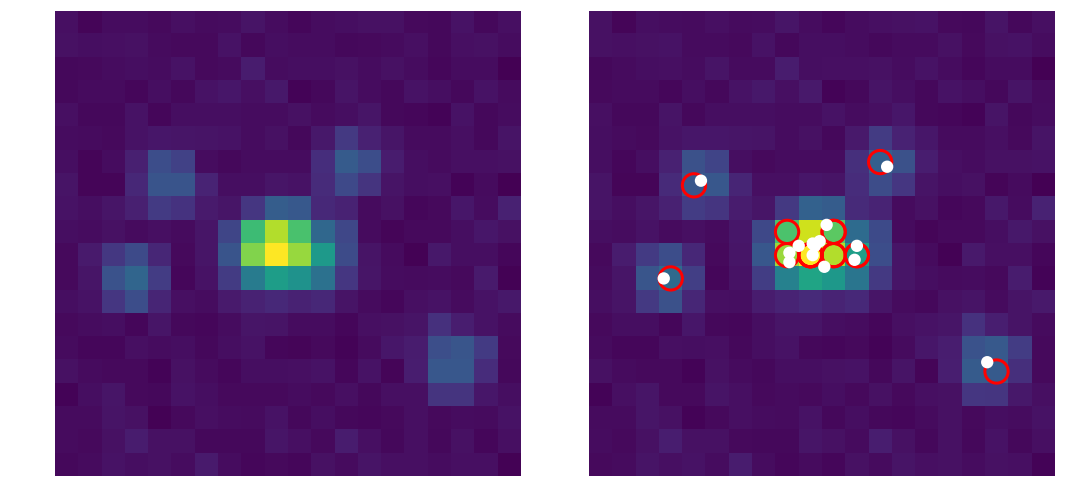
\includegraphics[width=1\textwidth]{figures/chapter2/plot_dense_decomposition}
    \caption{Detected (red) and actual (white) clustered spots}
    \label{fig:dense_decomposition}
\end{figure}

\subsection{Going beyond pixel accuracy} \label{subsec:subpixel}

Two additional methods already present in the first version of FISH-quant\cite{mueller_fish-quant_2013} have been implemented in \emph{bigfish} as it is.

\paragraph{Subpixel fitting}

So far, the spot detection and the dense region decomposition and the cluster detection return coordinates at the pixel level.
This can lead to a small inaccuracy, irrelevant for our own studies, but potentially critical for some users.
Such error can be observed in the figure~\ref{fig:dense_decomposition} between the detected spots (with a pixel accuracy) and the ground truth (with a subpixel accuracy).

The possibility to refine the coordinate on individual spots solves this limitation.
We simply loop over the detected spots, crop their image and fit a gaussian signal on each of them.
We then correct the spot coordinates with the coordinates of the fitted gaussian.
Obviously, such method might return negative results in high density areas when spots can't be resolved.\\

\begin{minipage}{0.9\textwidth}
\begin{lstlisting}[language=Python]
import bigfish.detection as detection

# subpixel fitting
spots_subpixel = detection.fit_subpixel(
    image=smfish,
    spots=spots,
    voxel_size=(300, 103, 103),  # in nanometer
    spot_radius=(350, 150, 150))  # in nanometer
\end{lstlisting}
\end{minipage}

\paragraph{Spot colocalization}

\begin{wrapfigure}{R}{0.35\textwidth}
  \begin{center}
    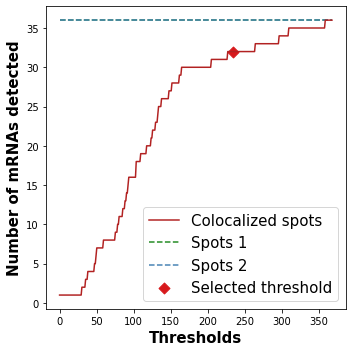
\includegraphics[width=0.33\textwidth]{figures/chapter2/colocalization_elbow}
  \end{center}
  \caption{Colocalization}
  \label{fig:elbow_colocalization}
\end{wrapfigure}

Another method requested by the community is the possibility to detect spots in two different channels then match their coordinates.
This could be the same \ac{RNA} detected with two different fluorescent probes or techniques.
For example in the figure~\ref{fig:elbow_colocalization} we detect colocalized spots between a sample of spots detected with a pixel accuracy and the same sample with a subpixel accuracy.

First we compute the euclidean distance matrix between the two sets of spot coordinates, then we solve a linear sum assignment problem\cite{crouse_linear_assignment_2016, 2020SciPy-NMeth}.
We obtain an matching between the two sets of spots, for each spots, that minimize the overall euclidean distance between assigned pairs.
Finally, we only keep pairs with a distance below a specific threshold.
The figure~\ref{fig:elbow_colocalization} illustrates the impact of the threshold parameter on the number of colocalized spots.
Like for the spot detection, we implement our heuristic~\ref{subsec:spot_detection} to infer an optimal threshold if none is provided.\\

\begin{minipage}{0.9\textwidth}
\begin{lstlisting}[language=Python]
import bigfish.multistack as multistack

# spot colocalization
(spots_1_colocalized, spots_2_colocalized,
 distances) = multistack.detect_spots_colocalization(
	spots_1=spots_crop,
	spots_2=spots_subpixel_crop,
	voxel_size=(300, 103, 103))  # in nanometer
\end{lstlisting}
\end{minipage}

\section{Evaluation with simulated spots} \label{sec:detection_evaluation}

This section describes how we evaluate the performance of \emph{bigfish.detection}.
In addition to qualitative assessment of spot detection throughout our studies, we quantify the accuracy errors with simulated images.
These simulations are produced with the \emph{simfish} package.

\subsection{Simulation} \label{subsec:simulation}

To measure the error of a spot detection we need a ground truth.
A manual annotation of a regular 3D \ac{smFISH} image is intractable.
It would be time-consuming and prone to human error.
The alternative is to simulate realistic images of spots, under different conditions to stress the performances of our algorithms.
To this end, \emph{simfish} allows us to precisely control the level of noise and the number of spots we want to simulate in the image.

\paragraph{Spot simulations}



\noindent
Our images are generated with three main steps:

\begin{enumerate}
	\item We randomly draw the number of spots and their localization in 3D.
	The number of spots is sampled from a Poisson distribution and the localizations from an uniform distribution all over the frame.
	Alternatively the number of spots can be set manually.
	The user can also decide to simulate clusters.
	In this case, the number of clusters and the number of spots per cluster are drawn from a Poisson distribution,
	\item
	\item
	\item
\end{enumerate}

\paragraph{\ac{Cluster}}


\paragraph{\ac{SNR}}


- snr
- spots
- noise
- cluster
- subpixel

- random distribution
- poisson distribution


In order to create ground-truth datasets for assessing localization performance,
we generated images simulating diffraction-limited spots in the following way: (𝑥, 𝑦, 𝑧) spot
positions were randomly assigned within the z-stack chosen dimensions, and each
spot was assigned a brightness picked from a normal distribution. We computed
the intensity 𝐼(𝑥, 𝑦, 𝑧) generated by each spot as follows: we first computed
the predicted average number of photons received by each pixel 𝐼*+,#
user-defined lateral and axial extensions. We then simulated the actual intensity
collected at each pixel using a Poisson-distributed value with mean 𝐼*+,#
gaussian-distributed noise to each pixel of the image.

%Simulated images to validate spot detection algorithms

%To evaluate our spot detection algorithm, we simulated 3D images with spots
%mimicking the smFISH signal produced by RNA molecules.




# get spots coordinates
scale_z = None
if ndim == 3:
	spots_scale_z = sigma[0] / voxel_size[0]
	scale_z = spots_scale_z * 0.2 * nb_spots_cluster
spots_scale_yx = sigma[-1] / voxel_size[-1]
scale_yx = spots_scale_yx * 0.2 * nb_spots_cluster
if ndim == 3:
	rho_z = np.abs(np.random.normal(
		loc=0.0, scale=scale_z, size=nb_spots_cluster))
	rho_yx = np.abs(np.random.normal(
		loc=0.0, scale=scale_yx, size=nb_spots_cluster))
	theta = np.random.uniform(0, np.pi, nb_spots_cluster)
	phi = np.random.uniform(0, 2 * np.pi, nb_spots_cluster)
	z = center_cluster_z[i] + rho_z * np.cos(theta)
	positions_z.append(z)
	y = center_cluster_y[i] + rho_yx * np.sin(phi) * np.sin(theta)
	positions_y.append(y)
	x = center_cluster_x[i] + rho_yx * np.cos(phi) * np.sin(theta)
	positions_x.append(x)

else:
	rho_yx = np.random.normal(
		loc=0.0, scale=scale_yx, size=nb_spots_cluster)
	phi = np.random.uniform(-np.pi, np.pi, nb_spots_cluster)
	y = center_cluster_y[i] + rho_yx * np.sin(phi)
	positions_y.append(y)
	x = center_cluster_x[i] + rho_yx * np.cos(phi)
	positions_x.append(x)





These images are obtained with three main steps:

%1. We randomly draw the number of spots (this parameter can also be predetermined)
%and their localization in three dimensions.

%2. For each spot we simulate a 3D Gaussian signal with a predefined amplitude and sigma.
%The final intensity of every pixel is sampled from a Poisson distribution with the gaussian simulated value as expectation.

%3. We simulate a background white noise over all the image, following a normal
%distribution centered around a predefined noise level.

figure~\ref{fig:spot_detection_high_noise}

\begin{figure}[h]
    \centering
    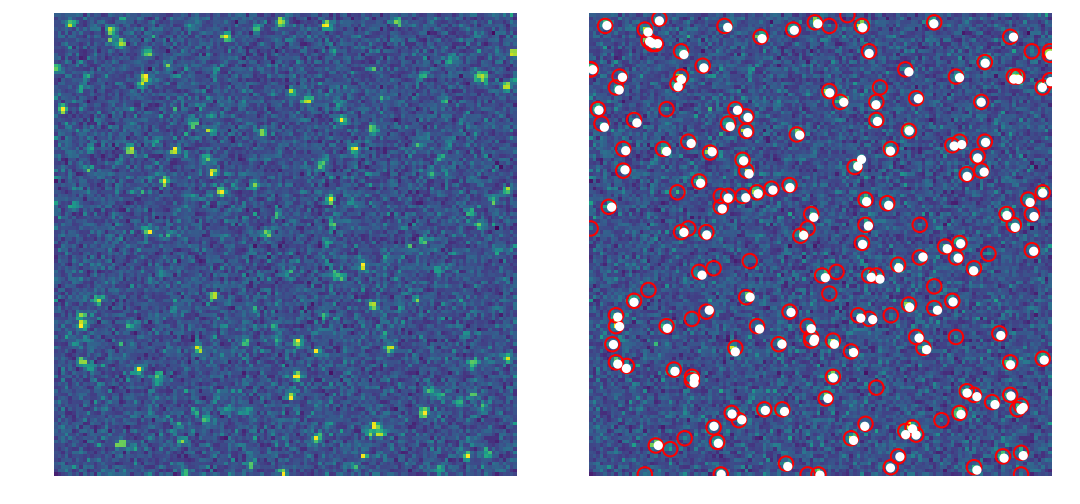
\includegraphics[width=1\textwidth]{figures/chapter2/plot_spot_detection}
    \caption{Detection of highly noisy spots}
    \label{fig:spot_detection_high_noise}
\end{figure}




To evaluate detection in imaging conditions with different noise levels,
we varied the parameters to simulate images. Signal quality was evaluated
with the Signal-To-Noise ratio (SNR). SNR is calculated for each spot, where
we define the background as a region surrounding its center and a radius
twice the size of the spot radius, with the following equation:

% equation

\subsection{Results} \label{subsec:detection_results}


% impact of SNR

\begin{figure}[h]
    \centering
    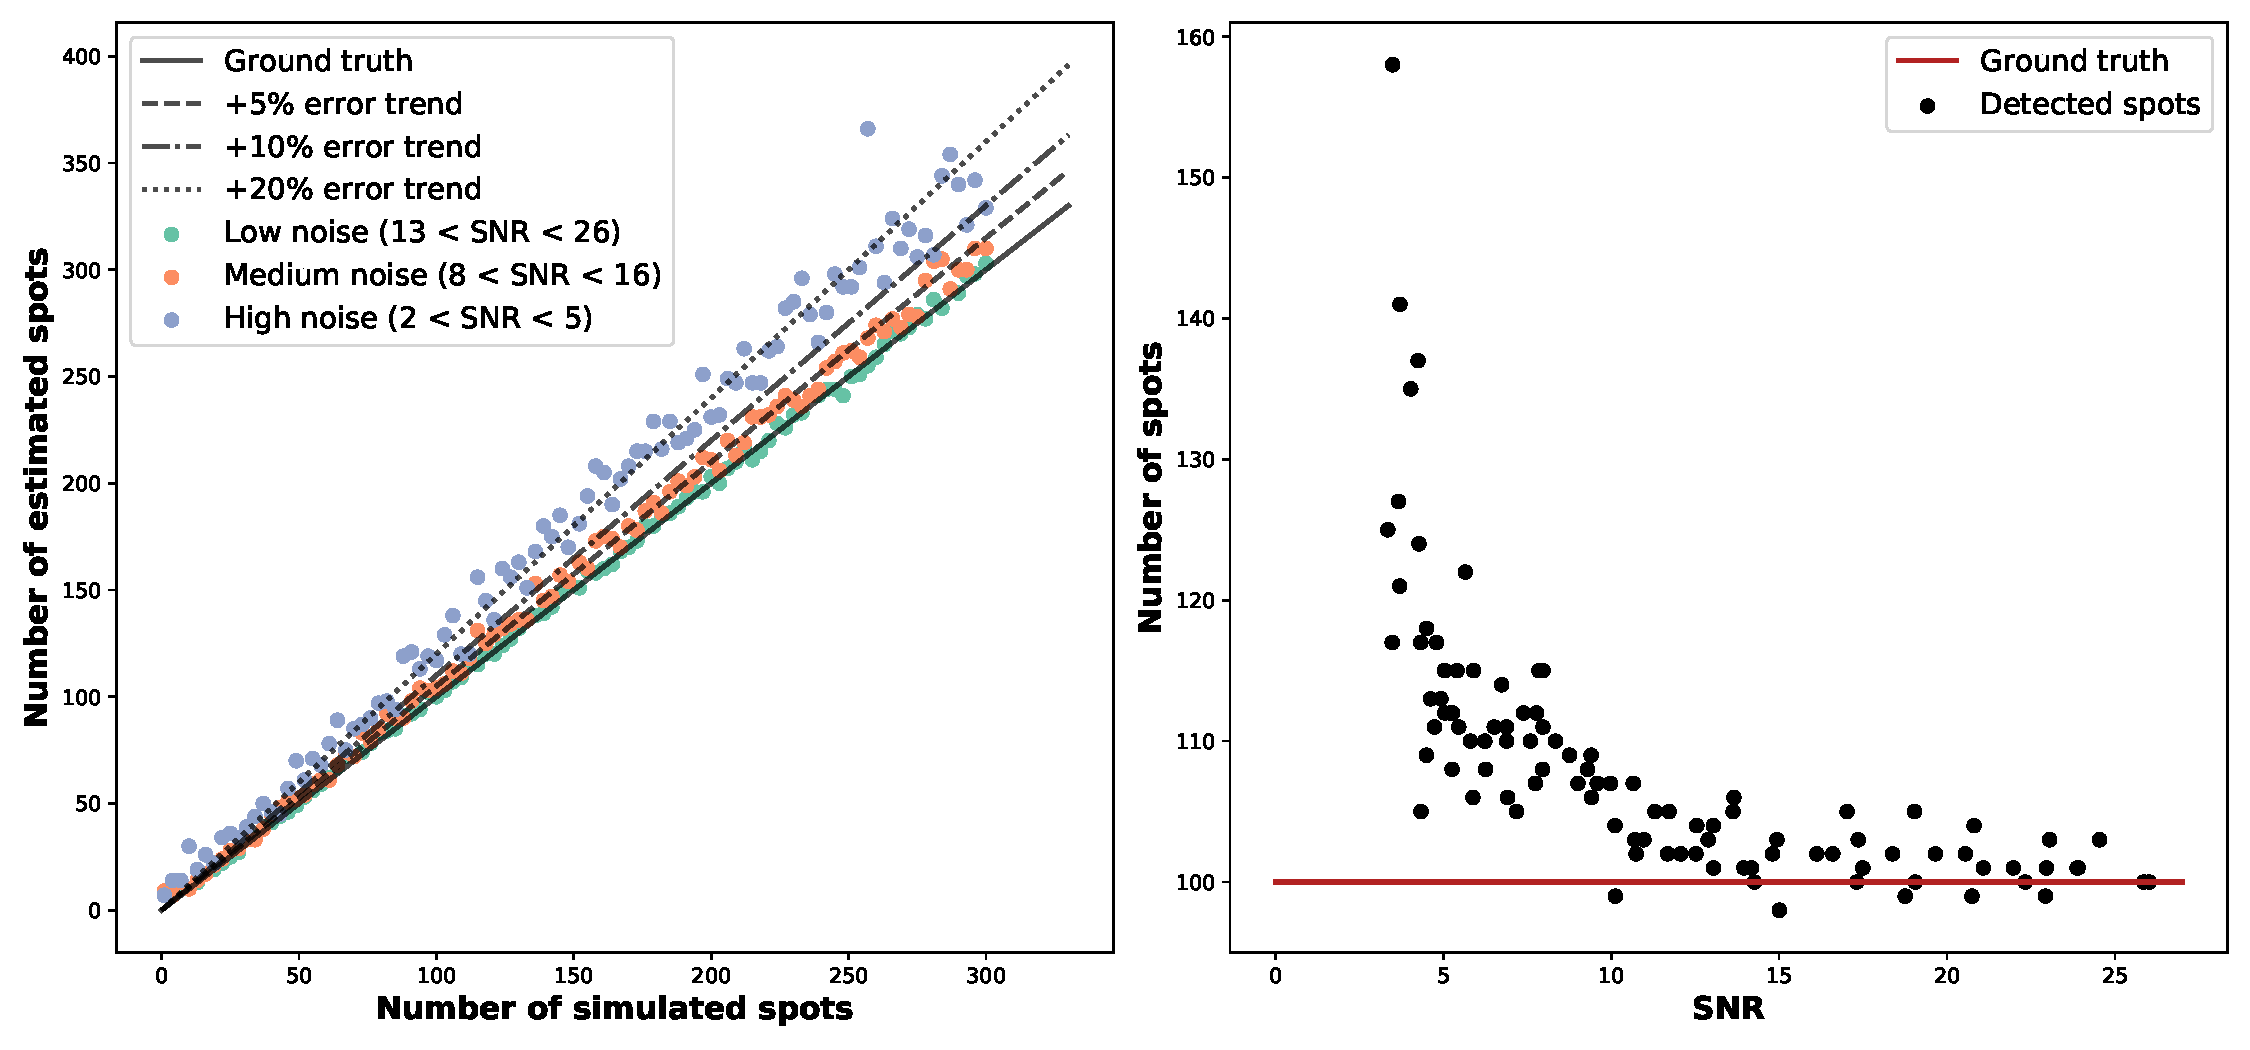
\includegraphics[width=1\textwidth]{figures/chapter2/fused_spot_detection_noise}
    \caption{Spot detection evaluation}
    \label{fig:detection_error}
\end{figure}

\begin{figure}[h]
    \centering
    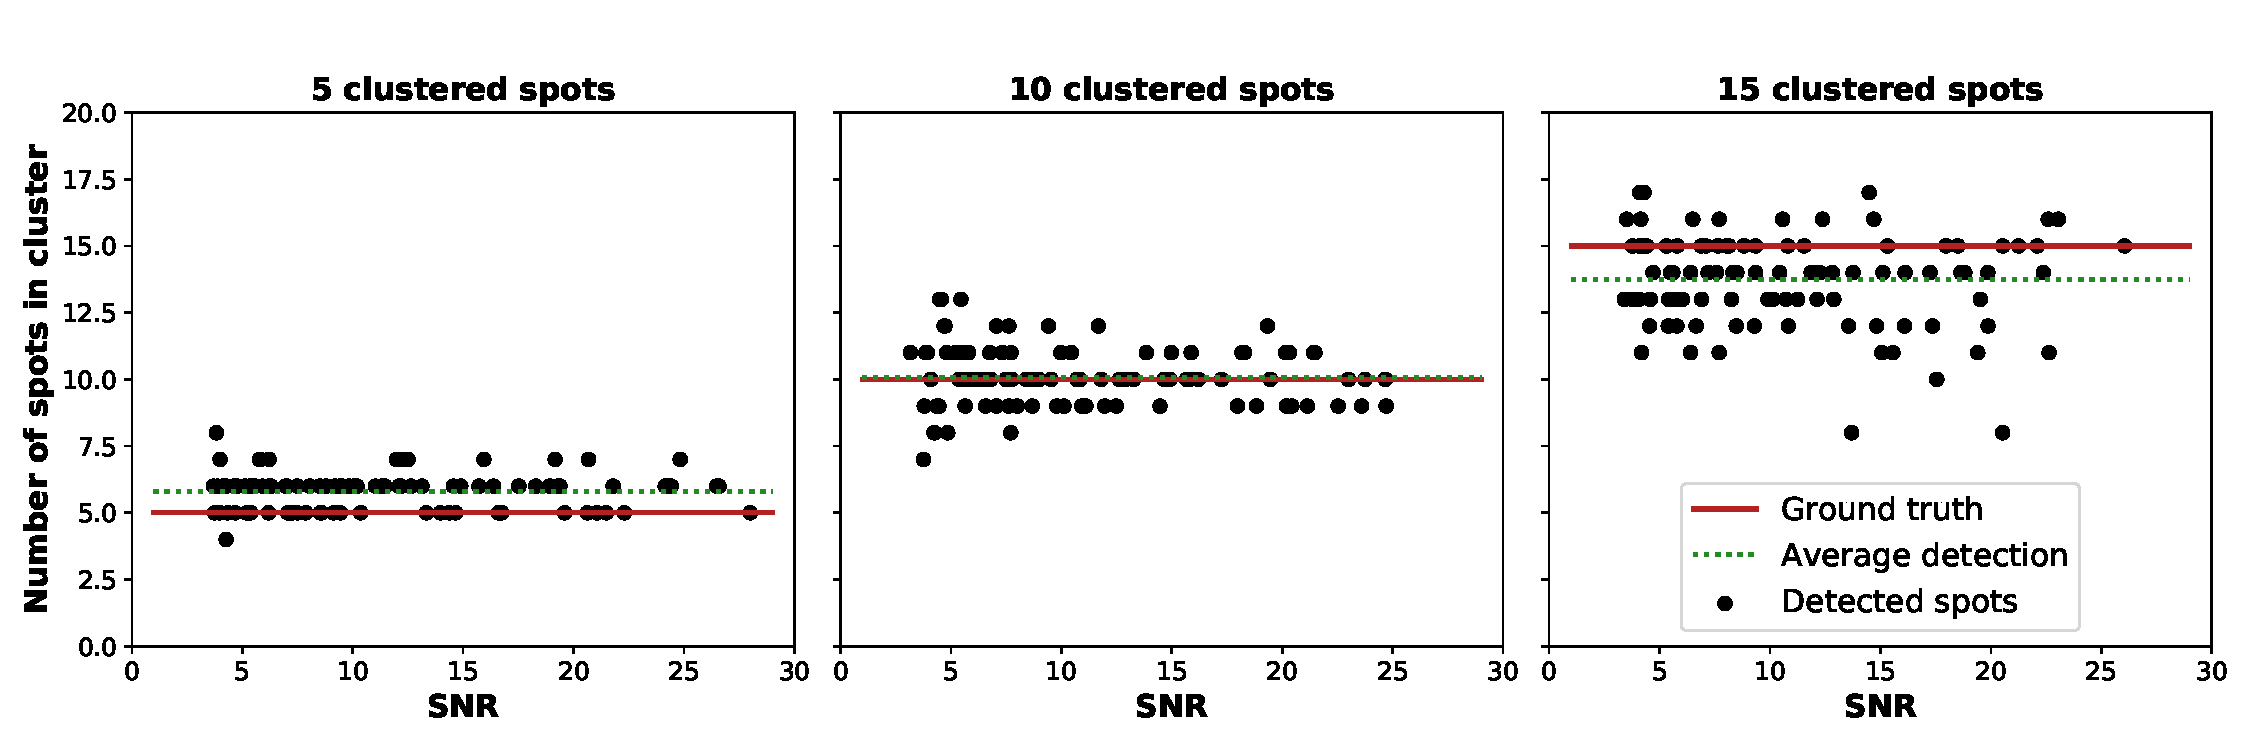
\includegraphics[width=1\textwidth]{figures/chapter2/cluster_along_noise}
    \caption{Dense region decomposition evaluation}
    \label{fig:cluster_results}
\end{figure}


\subsection{What if the \ac{PSF} is not a gaussian?} \label{subsec:psf}



\section{Conclusion} \label{sec:detection_conclusion}

The detection subpackage implements the methods re- quired to detect spots in
2D or 3D images (Figs. 2, 3A–E). An important aspect of the detection subpackage
is its abil- ity to detect spots without setting any pixel intensity thresh- old.
We implemented a method to automatically infer this threshold from the image.
The curve describing the num- ber of detected spots as a function of the
intensity threshold (Fig. 3A,B) has an elbow shape, resulting from the superposition
of the fast decreasing false positive de- tections (low intensity noise) and the
slowly decreasing true positives. The threshold selected corresponds to the kink
in the elbow, and corresponds thus to the highest threshold outside the high-noise
regime. In order to val- idate this approach, we simulated real- istic smFISH images
with varying noise levels (Fig. 3A,B; Supplemental Note 1). We found that our method
only leads to a moderate over-estimation of detected spots (<5%–10%) for images with
moderate to high SNR values (>5). Such automatization over- comes human intervention
and allows scaling to large data sets, such that the subpackage can process thousands
of images. While initially designed to detect individual mRNAs, the same methods
can also be used to detect other spot-like structures (Safieddine et al. 2021),
such as centrosomes, P- bodies, etc (Fig. 3E).This subpackage further permits us
to perform localiza- tion of RNAs with subpixel accuracy by using a Gaussian
fitting (Mueller et al. 2013). Lastly, we provide the pos- sibility to perform
a colocalization analysis between spot detection per- formed in multiple channels (Cornes et al. 2021).

% https://github.com/PreibischLab/RS-FISH/tree/master/documents/tool_comparison_for_paper